% 
% Annual Cognitive Science Conference
% LaTeX Paper -- Proceedings Format
% 

% Original : Jin-Hwa Kim (jhkim@bi.snu.ac.kr)        06/02/2014
% Modified : Jin-Hwa Kim (jhkim@bi.snu.ac.kr)        06/22/2014

%% Change ``a4paper'' in the following line to ``letterpaper'' if you are
%% producing a letter-format document.

\documentclass[10pt,letterpaper]{article}

\usepackage{cogsci}
\usepackage{pslatex}
\usepackage{apacite}

\usepackage{nameref}
\usepackage{graphicx}

\title{Active Long Fixation Correlates with the Formation \\
of Long-Term Memory}
 
\author{{\large \bf Jin-Hwa Kim (jhkim@bi.snu.ac.kr)} \\
  Cognitive Science Program, Seoul National University \\
  Seoul, 151-742, Republic of Korea
  \AND {\large \bf Byoung-Tak Zhang (btzhang@bi.snu.ac.kr)} \\
  School of Computer Science and Engineering, Seoul National University \\
  Seoul, 151-742, Republic of Korea}

\begin{document}

\maketitle

\begin{abstract}
The application of eyewear accelerates the study on the eye movement, for the eye movement is a non-invasive and convenient indicator of the brain activities. We investigate the eye movements of the subjects watching the kids video. We analyze the video sequences by classifying into two different sequence groups have the long and short fixation duration, respectively. First, we conduct the long-term memory test of whether fixation duration correlates with long-term memory. Second, we classify its visual constraints into Alert and No Alert types. As a result of the test, the fixation duration itself is not decisive, however, the long fixations which are actively engaged with Alert type sequences statistically have higher recall scores, but the short fixations do not. Finally, we tentatively propose a computational model for the embodied cognitive framework with the perception-action cycling, which may provide an explanatory way to the efficient memory mechanism for the life-long sequences.

\textbf{Keywords:} 
Eye movement; fixation; spatio-temporal; long-term memory, computational modeling.
\end{abstract}


\section{Introduction}

The brain is the most intelligent organ of a living thing. It receives many different forms of sensory information and processes this information appropriately with regard to its survival and reproduce. Especially, the visual information takes a very special position among other kinds of sensory information as it does not need to sense a source directly but is transfered to a remote target far freely than any other types of the sense. Furthermore it gives more chance to survive in the situation of being threaten by the predators using the eyes to detect the foes in the remote place before their approaching. 

But this notable advantage is not freely given one as it requires more delicate and clever way of interpreting the visual information. Because the visual information can easily be affected by the moment-to-moment environmental changes, heuristic but robust compensation strategies are demanded. Hence, how the brain processes the visual information provides the profound way to study the mechanism that the brain precisely and efficiently processes the most dynamic and enormous sensory information.

There are a lot of studies on the computational modeling for the visual information, which include the visual fragment completion, the scene or object classification and recognition \cite{winn2005,lazebnik2006}, and object tracking \cite{YiWu2013}. These research topics often tend to focus on the objective for each task, not on the implementation of the method how the brain deals with. As a result, the computational approach to the modeling for the visual information processing of the brain is gradually changed to the optimization problem, which hinders the understand of the human-level information processing abilities. 

Particularly, the object tracking seems to describe how we pay attention to an interesting object, however, the eye movement mostly controlled by the oculomotor system, is more complicated how the brain works for the acquisition of the visual information \cite{Henderson2003}. For instance, in the fixation state, the human eyes only recognize the small portion of the whole sight. If you read this paper from an 8-inch distance fixing on one particular letter, you cannot read outside of next two words or about ten letters which are presented in the para-fovea. For the brain is well-known for its parallel processing on the neural circuits, this sequential notion of eye movement for the visual system would be inefficient for information processing.

The studies on the reading eye movement, which are relatively well studied by psychologists and neuroscientists \cite{Rayner1998,Reichle1998}, reveal the fixation duration is related to the presence of the cognitive process \cite{Rayner1997}, for an instance, observing its correlation with linguistic attributes \cite{Inhoff1986,Rayner1986}.

There is a different aspect of studying on the eye movement for video stimuli. How long the fixation sustains is more constrained by the affective content, i.e. emotional response, context of the content, rather than the reading materials do. And the selection of the next fixation and the direction of a saccadic movement tend to be more liberal than the dominance of horizontal searching of reading does. 

Therefore, the study of the eye movement on the video stimuli has been neglected or avoided due to the research complexities and the methodological difficulties \cite{Tatler2011}. However, the recent advancement of the sensory device, like the Google Glass and the mobile devices for the eye tracking, promotes to study on the video stimuli and even more natural experimental environment, and to implement the research model or applications on those mobile devices. 

We investigate the characteristics of eye movements toward the video stimuli. The basic elements of the eye movements are segregated into the fixation duration and the saccade vector, which consists of the saccade direction and the length of the saccadic movement \cite{Findlay1999,Feng2006}. In this study, we focus on the characteristics of the fixation duration as the evidence of the cognitive process. Moreover, as the sequences which potentially induce the emotional arousal are known for helping to recall the seen movie clips \cite{Cahill1996amyg,Cahill1998baso}, we will see if the arousal effect is asserted by the duration of fixation.

\section{Materials and Methods}
\label{sec:material-and-methods}

\subsection{Experiment 1}

For this study, we prepared the video material \textit{Pororo Season 3}, which is a famous kids video in Republic of Korea. In this video, there are artificial 3D-rendered characters who have marked individualities. \textit{Pororo Season 3 DVD 1} contains the 13 consecutive episodes that each has a single storyline.

We recruit 18 participants with normal vision (11 males, 6 females; 23-31 years of age; median is 25), who are voluntarily participate in the study. All participants had not experienced a brain damage or a behavioral disorder. The participants are new to the video, \textit{Pororo Season 3}. Experimental procedures were agreed by the Research Ethics of Seoul National University and the participants signed a consent form.

Participants watched the kids video in the room which has the experimental settings. The room is about 3 square meters surrounding by the opaque curtains. On the side of the room, an wide-screen HDTV (1920x1080 resolution, 885 mm x 500 mm, 16:9 ratio) is installed, and 2.1 channel speakers. Participants are guided to sit down on the comfortable sofa in front of 1.7 m from the TV screen.

Concurrently, the eye movements and the user-perspective scenes are recorded by \textit{Tobii Glasses eye tracker}, the corneal reflection based system with a sampling rate of 30 Hz. We used the \textit{I-VT algorithm} as the fixation filter (system default), which classifies fixations with the velocity threshold, 30 degree per second. Usually, the saccadic eye movements are discriminated with low velocities (less than 100 degree/second) and high velocities (higher than 300 degree/second), so the velocity-based classification is simple but reasonable approach \cite{Salvucci2000}.

We classified the event types of the eye movements into three categories; fixation, saccade and unclassified. The unclassified data is discarded and not used in this study.

\begin{figure}
  \centerline{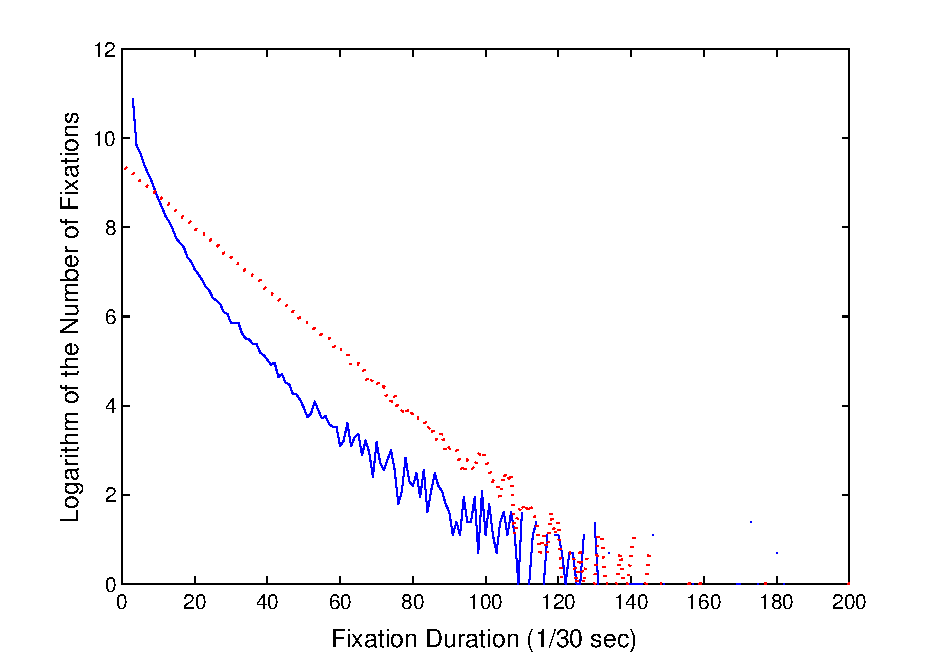
\includegraphics[width=86mm,trim=10mm 3mm 10mm 3mm]{./eps/marginal_fixation_duration.pdf}}
  \caption{The marginal distribution of fixation durations. All of the 158,643 fixation durations of 18 participants is used. The x-axis represents the number of time unit, 1/30 sec., therefore, 30 indicates 1 second. The y-axis represents the logarithm of the number of fixation which have the same time length with regard to the time unit of x-axis.}
  \label{fig:marginal-fixation-duration}
\end{figure}

\begin{figure}
  \centerline{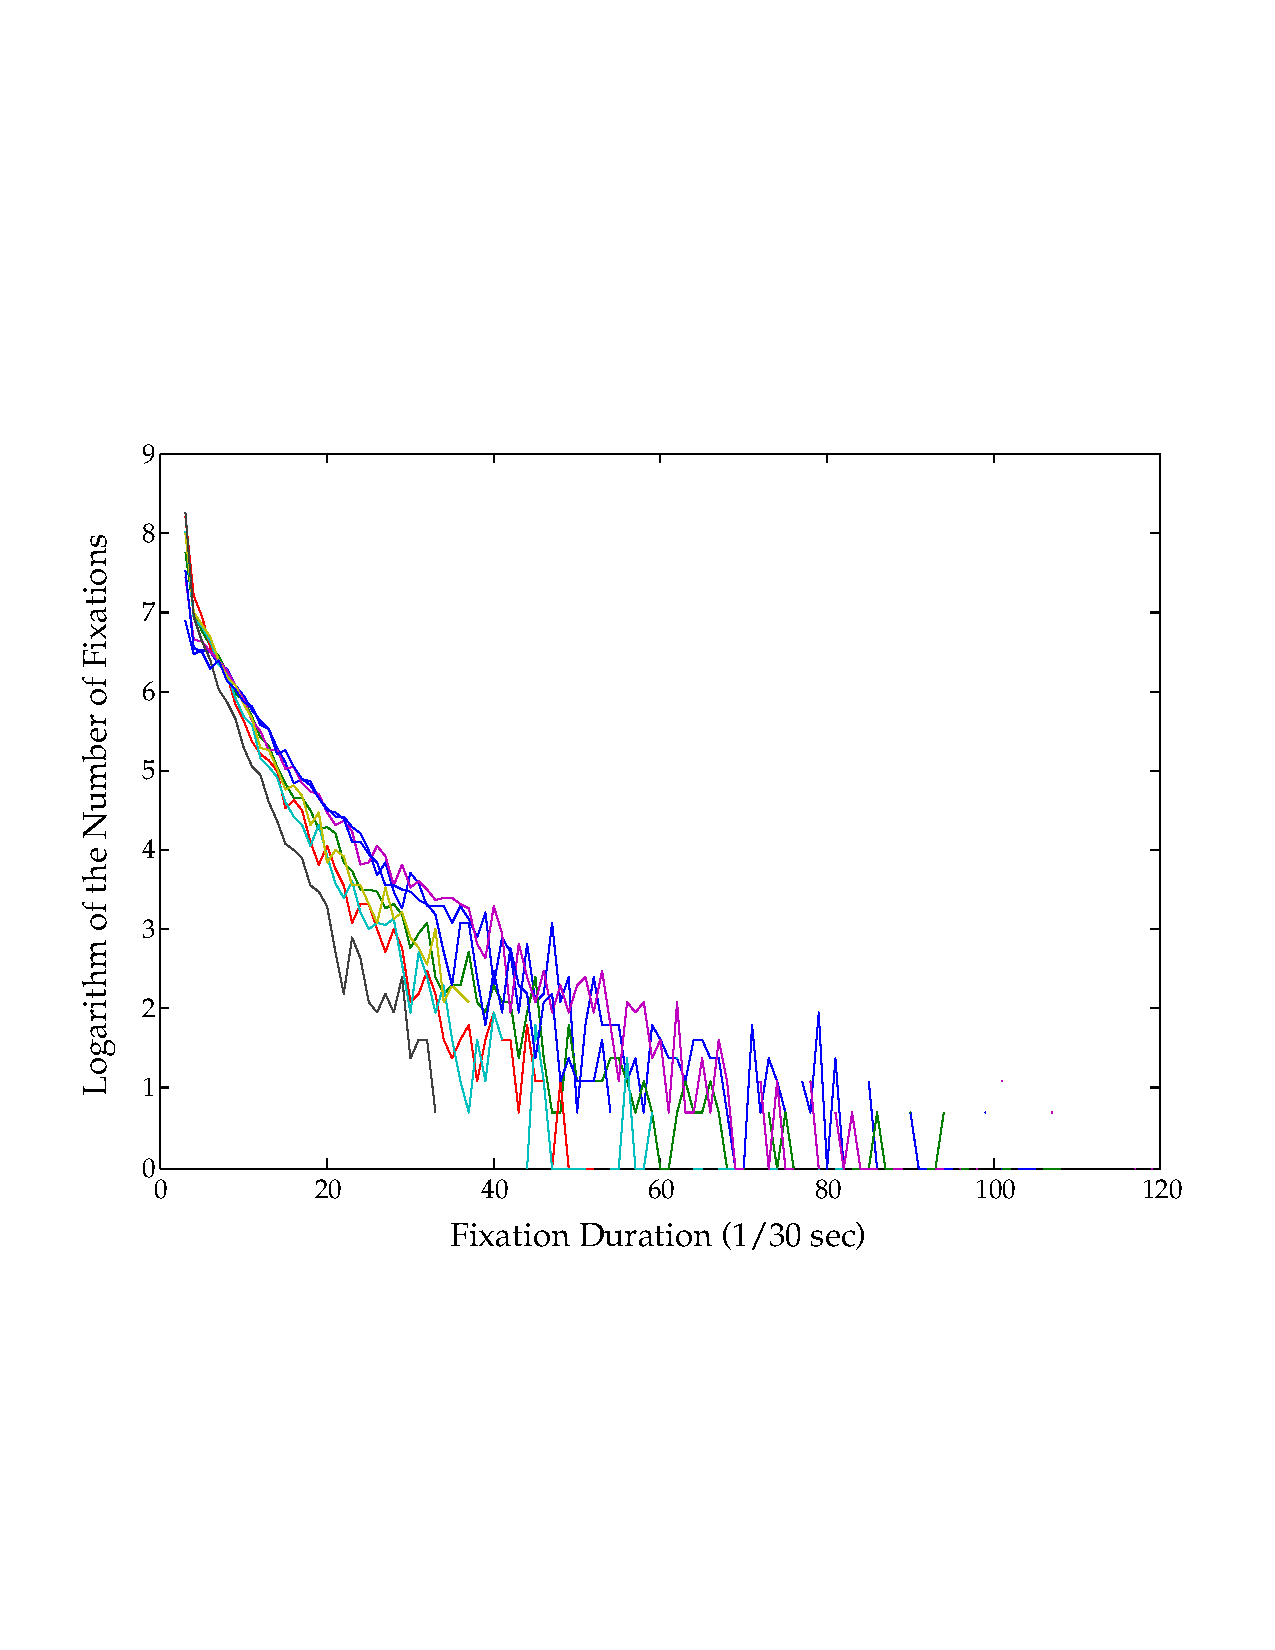
\includegraphics[width=86mm,trim=10mm 3mm 10mm 3mm]{./eps/individual_fixation_duration.pdf}}
  \caption{The distribution of fixation durations for the randomly selected 8 participants. We find the interpersonal differences among all 18 participants, the median of fixation durations varies from 133 ms to 267 ms (mean=183.3, std=41.7).}
  \label{fig:individual-fixation-duration}
\end{figure}

\subsection{Experiment 2}

For 11 participants who have participated in \textit{Experiment 1}, we prepared the controlled memory test for each participant. We conducted this experiment 3-4 months later after \textit{Experiment 1} (the intervals are not consistent due to schedule conflicts). A memory test consists of total 20 video sequences; 8 sequences for long fixations, another 8 sequences for short fixations, and the remaining 4 sequences for the control, which are not seen in the previous experiment. In detail, the lengths of all video sequences are the same as 3 seconds. \textit{The long fixation sequences} are randomly picked from each participant's data containing the fixation longer than 1400 ms in the middle of the sequence. \textit{The short fixation sequences} are randomly picked from each participant's data containing the fixation shorter than 300 ms. The 4 control sequences are randomly picked from the other season of \textit{Pororo} series, \textit{Pororo Season 2}.

Each participant identifies 20 sequences randomly sorted. Each participant gives a sequence 1 to 5 score depending on the assurance of whether he or she saw the sequence before or not. 

\section{Fixation Duration}
\label{sec:fixation-duration}

Fixation duration takes a important position in the reading literature as the duration of eye fixations seems to be constrained by the linguistic features of the fixated word \cite{Rayner1986,Inhoff1986}. In the video watching task, we anticipate the characteristics of fixation duration are different from that in the reading task. As we expect, the fixation duration changes more drastically, up to 10 seconds during watching the video. These changes are partly caused by the sequential changes of the visual stimuli and the fluctuated responses of the oculomotor system and cognitive processes. The length of fixation duration is not a deterministic property, because more than a single component dynamically contribute to the final motor command and the execution for the oculomotor system, we assumed the fixation duration as the random variable with probabilistic distribution \cite{Rayner1998,Reichle2004,Reichle2006}.

\subsection{Marginal Distribution of Fixation Durations}

Figure~\ref{fig:marginal-fixation-duration} shows the marginal distribution of fixation duration, which includes all of the 158,643 fixation durations of 18 participants. The x-axis represents the duration time, and the y-axis represents the log scale of the number of fixation durations across the whole data.

The shape of the marginal distribution of fixation duration (Figure~\ref{fig:marginal-fixation-duration}) can be illustrated with the exponential function (see the logarithm of the y-axis and the approximation plotted with red dotted line). While the distribution of the \textit{reading} fixation durations has a quiet different shape \cite{Feng2006}. The shape is roughly segmented into three parts, slow-rising ones for short fixations, fast-rising period until around 180 ms, and following a long tail for long fixation durations. These facts allow us to think that 180 ms of the fixation duration for reading is the most general case, but obviously not for watching the video.

Fixation durations which are longer than about 2 seconds are getting more unpredictable along with increasing the fixation duration. Though it is due to the logarithm increasing the sampling variance, occasionally the content of the video stimuli determines how long the eye gaze is fixated. In other words, the fixation more tends to maintain the gaze position when the visual constraint imposes. Surprisingly, the visual constraints have more various forms than we expected.

\subsection{Individual Distributions of Fixation Durations}

Interpersonal differences are also examined. The individual distributions of fixation durations are shown in Figure~\ref{fig:individual-fixation-duration}. For the simplicity, it only shows a handful portion of the participants'. The medians of fixation durations from all 18 participants varies from 133 ms to 267 ms with the mean is 183.3 and the standard deviation is 41.7.

\begin{figure}
  \centerline{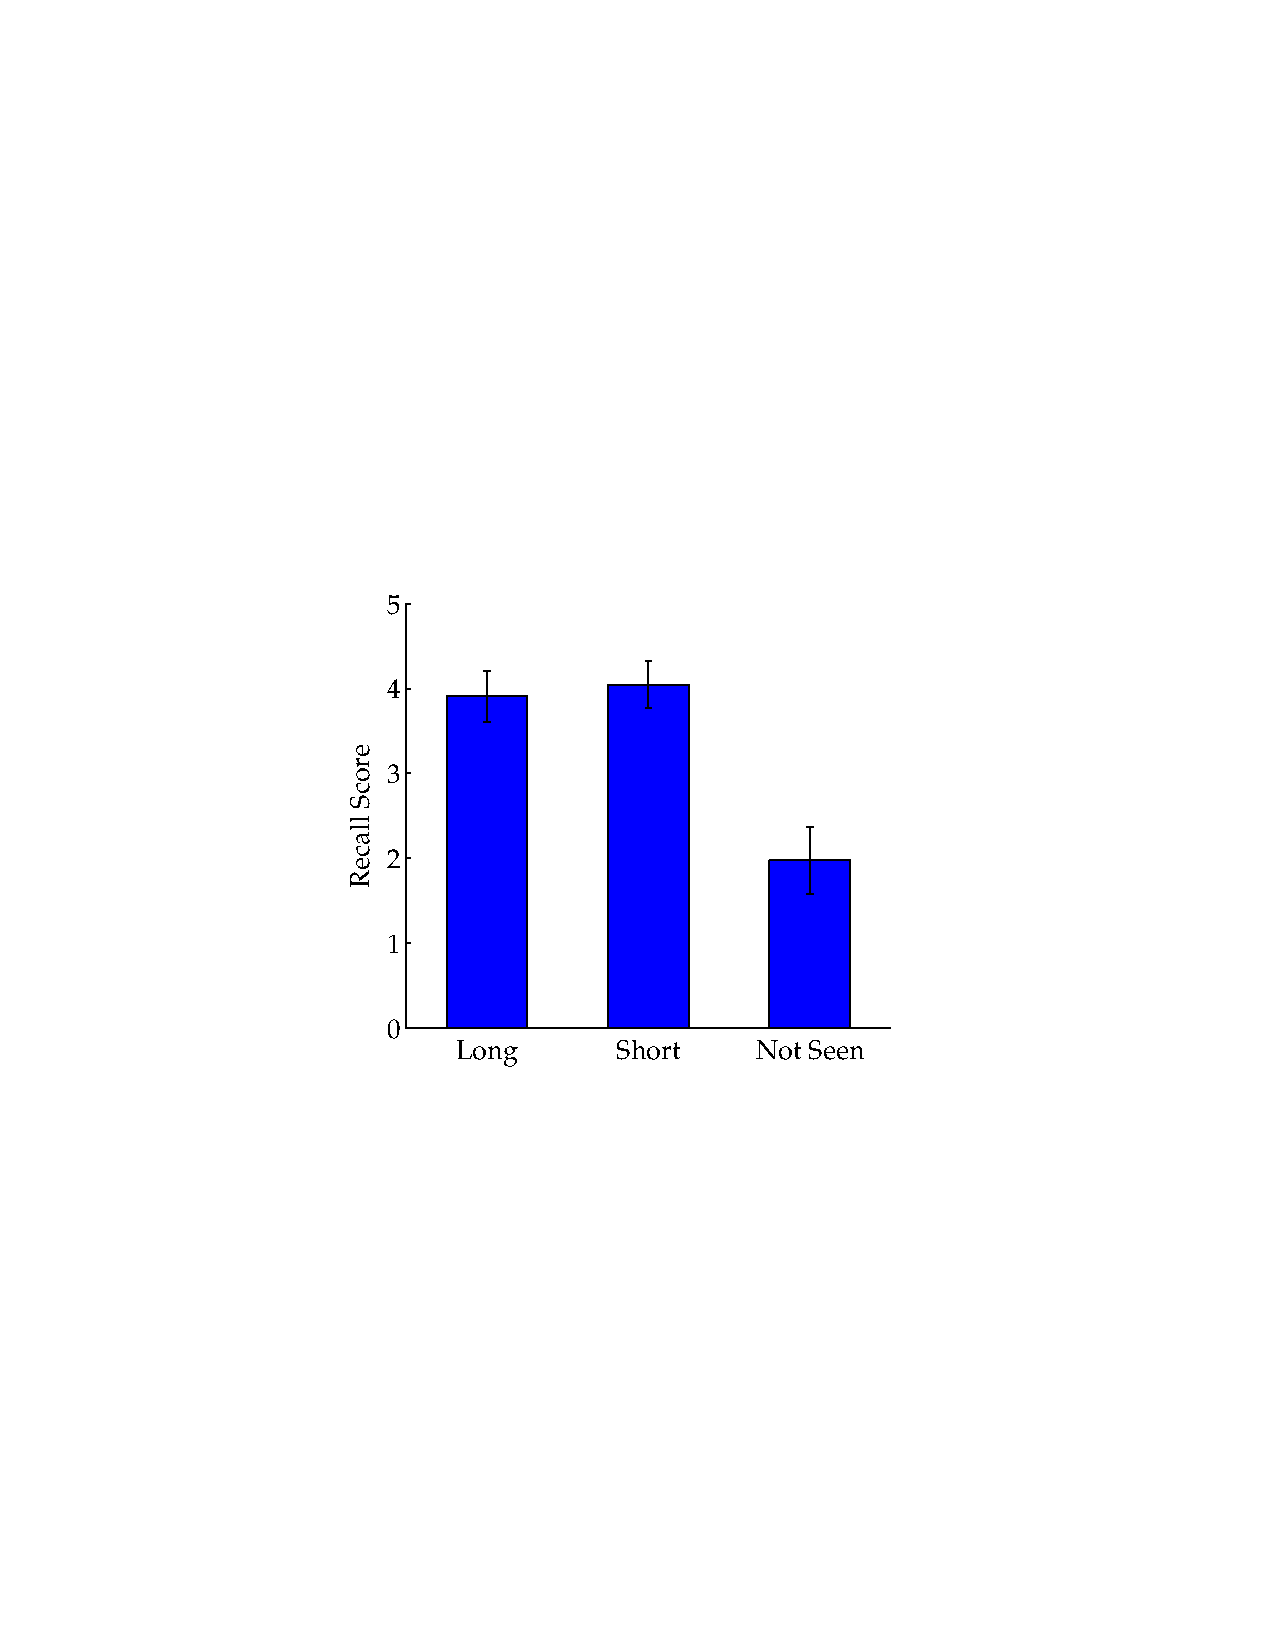
\includegraphics[width=60mm,height=54mm,trim=65mm 103mm 68mm 100mm]{./eps/memtest_leng}}
  \caption{Long-term memory test result for two fixation types, one is that whose duration of fixation is longer than 1400 ms, and the other one is that whose duration of fixation is shorter than 300 ms. Each participant rates 8 long fixated sequences, 8 short fixated sequences and 4 control sequences which are not seen previously. Surprisingly, the mean scores of the short fixated sequences is indifferent to the mean scores of the long fixated sequences (p $=$ 0.5051). Error bars indicate $\pm$ 2 standard errors of means (SEMs). For the detail of test, refer to \textit{\nameref{sec:material-and-methods}}.}
  \label{fig:memtest-leng}
\end{figure}

\begin{figure*}
  \centerline{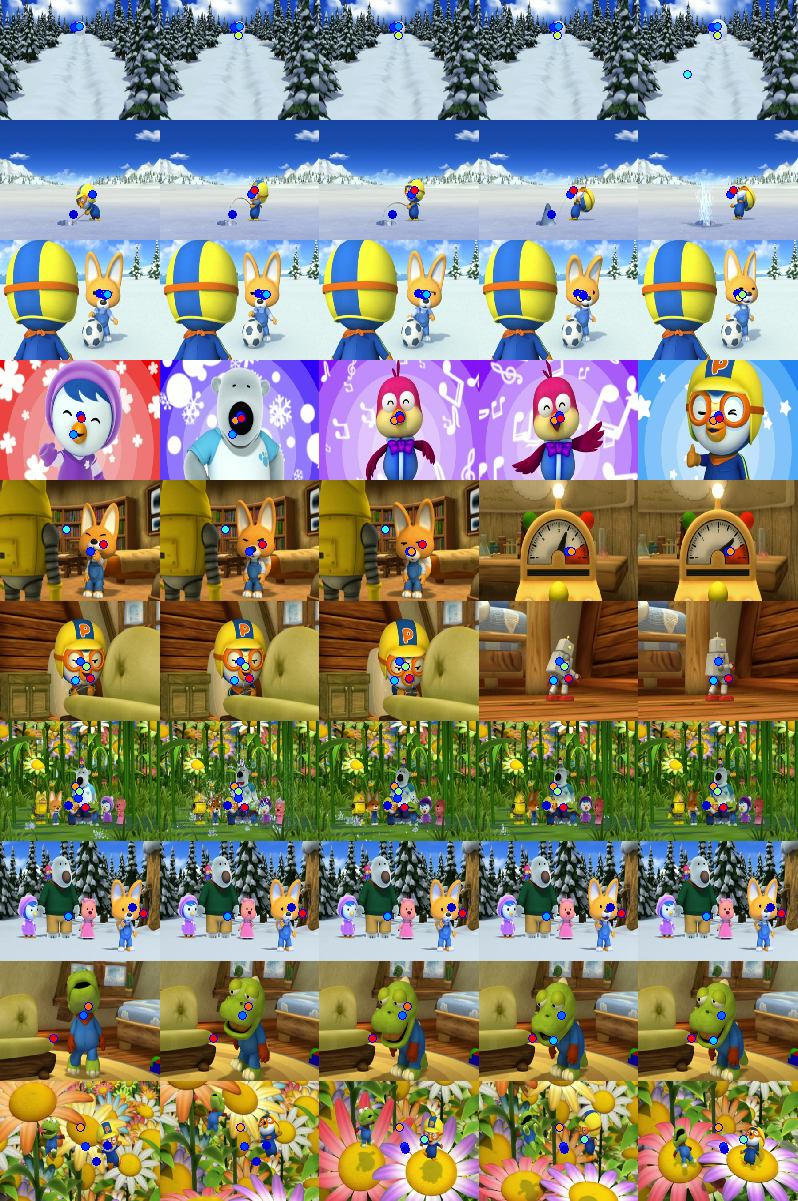
\includegraphics[width=120mm]{./eps/long_fixations_types.png}}
  \caption{The sequences of frames which receive more than 2 seconds of the fixation duration from at least 3 participants. Each row means the independent sequence and each column means the single frame. The time interval between the frames is 500 ms. The colored dots mean the fixation positions, whose durations are longer than 2 seconds. The same color means that which is from the same participant. First 3 sequences show the \textit{Alerted} type, then next 3 sequences show the \textit{Successive} type, then next 3 sequences show the \textit{Stationary} type, and then the last sequence shows the \textit{Unclassified} type of visual constraints for the review. For the description of those sequences, see the text in subsection~\textit{\nameref{subsec:Long-Fixation-Durations}}.}
  \label{fig:long-fixations}
\end{figure*}

\begin{table*}[!ht]
\begin{center} 
\caption{Long Fixation Types.} 
\label{tab:long-fixation-types} 
\vskip 0.12in
\begin{tabular}{ll} 
\hline
Long fixation type    &  Description \\
\hline
Alerted         &   An urgent situation happens with an object, 
                      which can be easily targeted as a cause. \\
Successive      &   Successive changes to keep attracting. \\
Stationary      &   The scene is the same while the target object(s)
                      moves a little or even does not move. \\
Unclassified    &   Cinematic techniques, which are tracking, tilt, 
                      zoom-in and out, and others. \\
\hline
\end{tabular} 
\end{center} 
\end{table*}

\subsection{Long Fixation Durations}
\label{subsec:Long-Fixation-Durations}

In Figure~\ref{fig:long-fixations} the sequences of frames which receive more than 2 seconds of the fixation duration from at least 3 different participants are shown. We set the threshold as 3 long fixations from the participants to reduce the interpersonal variation. We got all 41 sequences across 1 hour 7 minutes 50 seconds length of the material. For the review, we chose 10 typical sequences. Each row means the independent sequence and each column means the single frame. The time interval between the frames is 0.5 seconds. The colored dots mean the fixation positions, whose durations are longer than 2 seconds. The same color means the same participant. Four different types of the sequences are listed as \textit{Alerted} (3), \textit{Successive} (3), \textit{Stationary} (3), and \textit{Unclassified} (1) for the review.

The sequences of the \textit{Alerted} type are classified as the scene implies an unusual or potentially dangerous or difficult situation, which may introduce a mental arousal. The sequence of first row demonstrates an urgent moment that a huge snowball is about to roll down back the hill, which was previously rolled up by the robot \textit{Rody}. Second shows that \textit{Pororo} was fishing at the ice hole, but what he caught was \textit{Shark}, a naughty character. Third shows that \textit{Eddy} rolled his eyes to kick his ball avoiding the opponent \textit{Pororo}.

The \textit{Successive} type shows that the fixation extends across more than 2 different scenes. Because the location of the target object is not changed or changed within the range of a foveal or central vision, 2-5$^{\circ}$, the fixation holds its position \cite{mcmorris2014acquisition}. The fourth sequence shows the close up characters are serially shown up in the middle of the screen. The fixations of the fifth and sixth sequences extends across 2 different scenes have a different visual configuration.

The \textit{Stationary} type most clearly shows the characteristics that the indifferent scene maintains while the target object moves a little bit or even does not move. As there is not a particular event or a change of the scene, the participants tend to fixate their gazes. See the seventh through ninth sequences.

The sequences of the \textit{Unclassified} type have various forms. The tenth sequence shows that \textit{Pororo} and \textit{Crong} just jumped out of the shoulder of the magician dragon \textit{Tongtong} who was flying in the sky. Two sunflowers spring \textit{Pororo} and \textit{Crong} into the sky in multiple times. But due to the perspective of the camera, the location of the two characters in the scene is almost fixed. Participants fixated their eye gaze on the middle of two characters while the background shifting up and down. In other cases, though not included in Figure~\ref{fig:long-fixations}, few cinematic techniques, tracking, tilt, zoom-in and zoom-out, are examples. But the number of these cases is so small compared to the other types, hence we classified all of them into the \textit{Unclassified}.

These various types of the long fixated sequences show that a naive approach to the predict the visual constraint which induces the long fixation using a single analytical method, like the salient feature detectors \cite{marr1980,canny1986} or the optic flow \cite{koenderink1986} would fail. The \textit{Successive} and \textit{Stationary} types can be estimated by using the combination of the appropriate feature detectors and the optic flow, and the temporal modeling of the. However, the \textit{Alerted} cannot be solved without the cognitive modeling for the scene comprehension, which is related to the emotion-based reaction. 

\begin{figure}
  \centerline{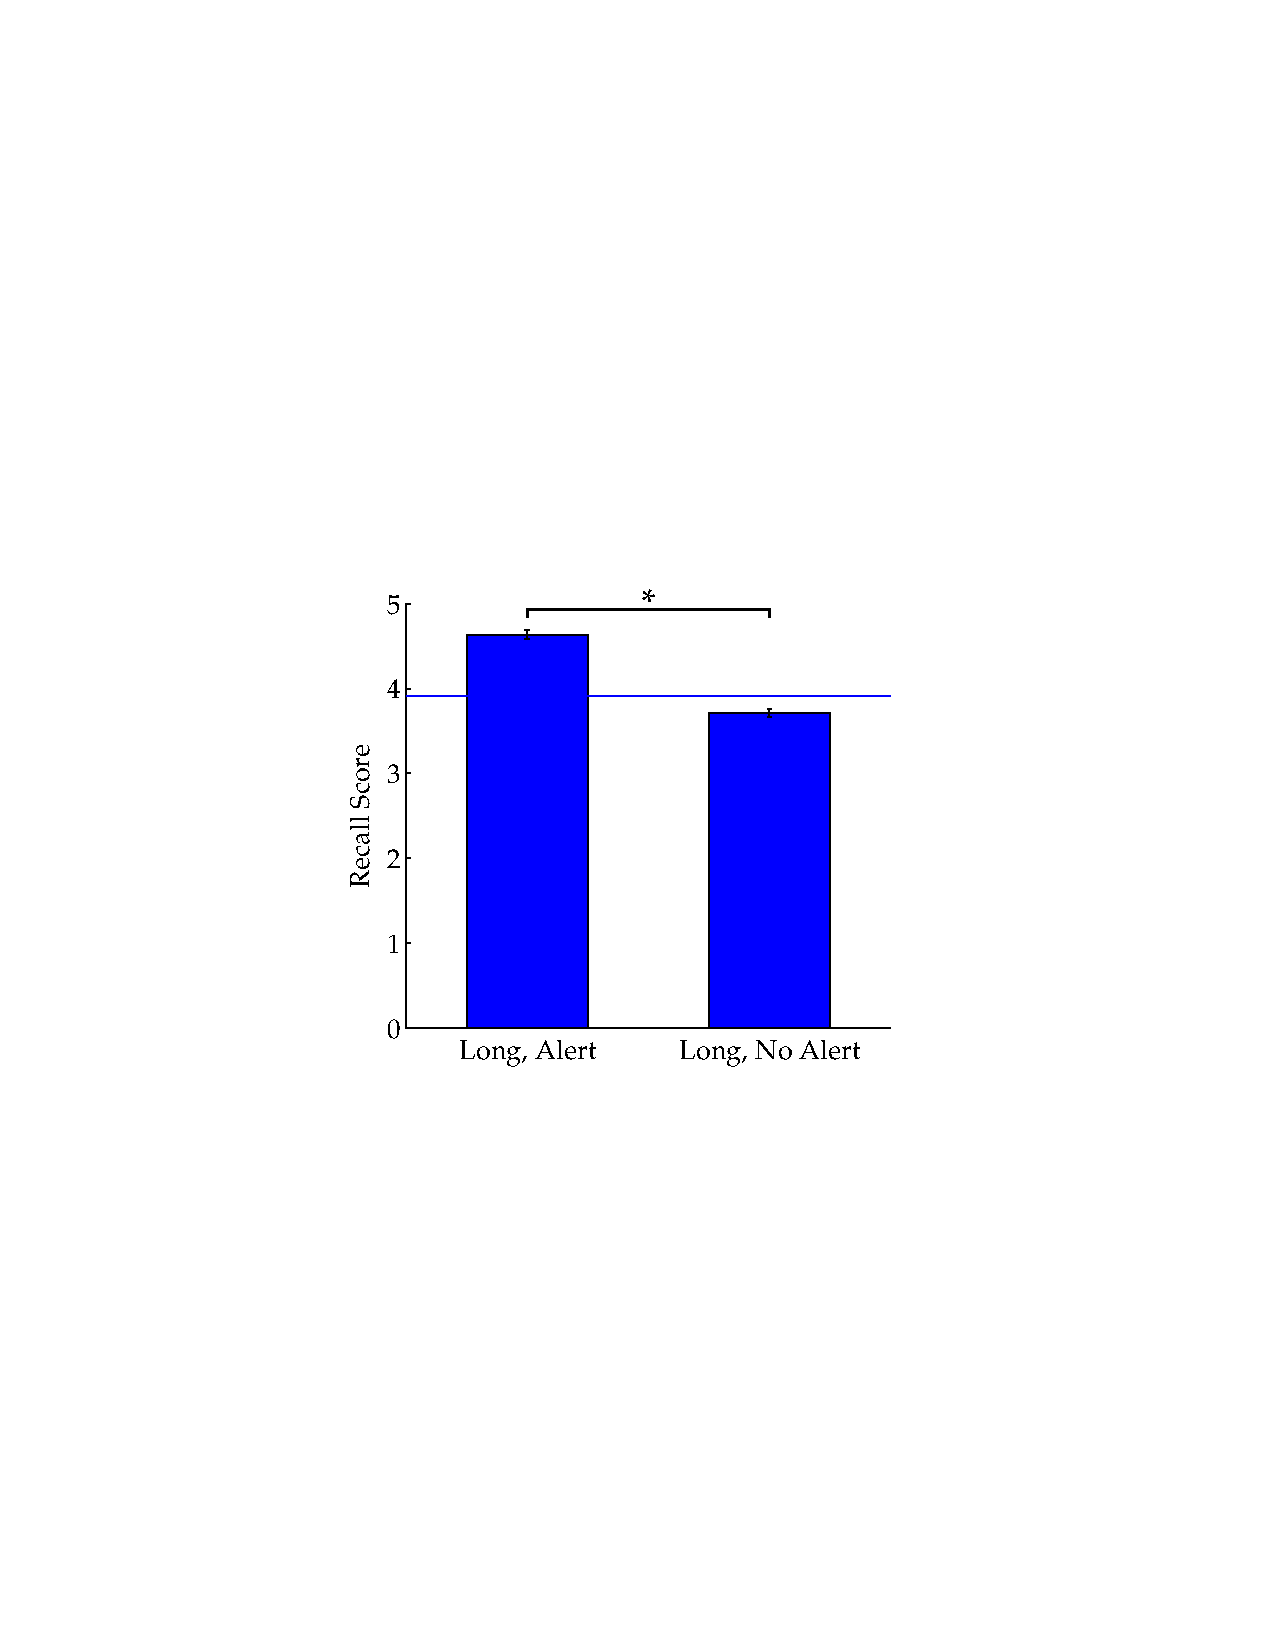
\includegraphics[width=60mm,height=54mm,trim=65mm 103mm 68mm 100mm]{./eps/memtest_long.pdf}}
  \caption{The memory test result for the \textit{long} fixation which is on the \textit{Alert} sequence or the \textit{No Alert} sequence. The number of cases from 11 participants are 19 and 69, respectively. The difference between two means is statistically significant, the p-value of two-sample t-test for the \textit{Alert} type is 0.0104 ($<$ 0.05). The blue horizontal line indicates the mean scores of the \textit{long} fixated sequences. Error bars indicate $\pm$ 2 SEMs.}
  \label{fig:memtest-long}
\end{figure}

\begin{figure}
  \centerline{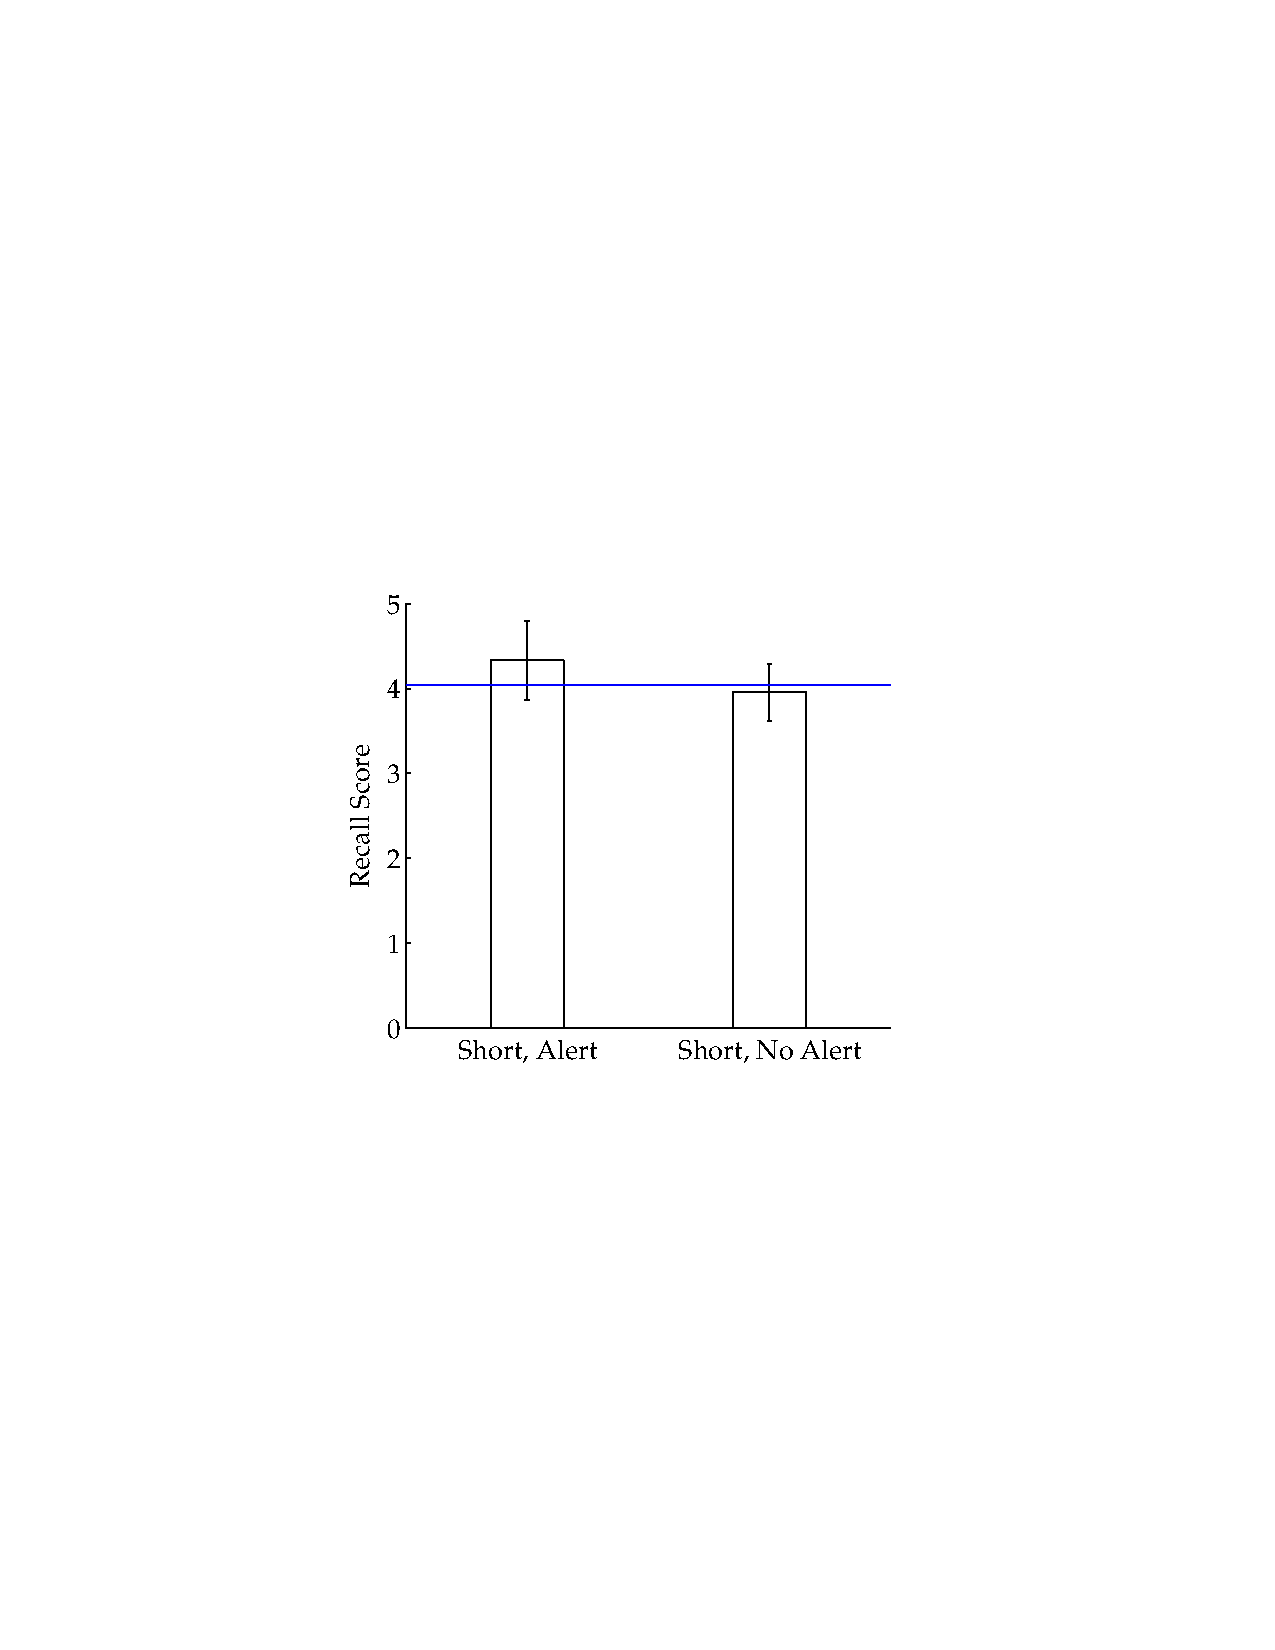
\includegraphics[width=60mm,height=54mm,trim=65mm 103mm 68mm 100mm]{./eps/memtest_short.pdf}}
  \caption{The memory test result for the \textit{short} fixation types which is on the \textit{Alert} sequence or the \textit{No Alert} sequence. The number of cases from 11 participants are 21 and 67, respectively. The p-value of two-sample t-test for the \textit{Alert} type is 0.2484 ($>$ 0.05). The blue horizontal line indicates the mean scores of the \textit{short} fixated sequences. Error bars indicate $\pm$ 2 SEMs.}
  \label{fig:memtest-short}
\end{figure}


\section{Long-Term Memory Formation}

In the studies of reading eye movements, as noted before, the fixation duration is a good indicator for the working of information processing. The stimulus-response model offers some way of understanding, because a sequence as a stimulus supplies a cause to response, in this case, a long fixation. But we have to be cautious as the long fixation itself is not always induced only when the internal state of a subject is positively affected. In addition, the sequences of long fixation does not decisively guarantee the quality of information processing nor its specificity as we carefully look into the sequences in Figure~\ref{fig:long-fixations}, which seems to include the sequences looking passively or even blankly. 

This view is also valid for the formation of memory. A stimulus is memorized by the constructive activities, a series of being stimulated, giving attention, and acquisition. But the corresponding response is not always guaranteed by the stimulus for environmental perturbations, noises or internal errors. Therefore, as the response is not decisive the formation of memory is the result of the cognitive process of response rather than the response itself. However, the cognitive process is an internal procedure, which only can be measured by the tangible responses indirectly. So, we need to discern the reliable indicator of the cognitive process with a sufficient care. 

The relationship between the emotional arousal and the formation of long-term memory is well established through the studies in neuroscience \cite{Cahill1996amyg,Cahill1998baso}. Based on that, we hypothesis that the formation of long-term memory correlates with the long fixation as an indicator of the cognitive process to emotional arousal stimuli. We also have the labed video clips whether it is emotionally arousal or not, we assume the stimuli is not decisive to induce the response. Moreover, we have to discern the response, the long fixation itself is a sufficient indicator for the formation of long-term memory. In this study, we define the emotionally arousal events are urgent, threat
tension, hurt, trouble, surprise or angry situations. Considering the video contents, happy or exciting events are prevailing and relatively short to cause the emotional changes.

We define two types of fixation as long and short fixations. The long fixation is the gaze holding its position after fixation filtering longer than 1400 ms. The short fixation is one that shorter than 300 ms. Figure~\ref{fig:memtest-leng} shows the memory test result for the two fixation types. Each participant assessed in a free recall test rating 8 long fixated sequences, 8 short fixated sequences and 4 not-seen sequences, which are not seen previously. Contrary to our expectations, the recall scores for the short fixated sequences is not much different from the the recall scores for the long fixated sequences. This result makes sense when we consider the possibility of that the long fixation as the response is an epiphenomenon.

The more detailed analyses are conducted constraining the type of stimuli.
Figure~\ref{fig:memtest-long} shows The memory test result for the \textit{long} fixation which is on the \textit{Alert} sequence or the \textit{No Alert} sequence. The \textit{Alert} sequences are classified by the predefined conditions, an unusual or potentially dangerous or difficult situation, which may introduce an emotional arousal. This classification is rather definite because the material is an animation video for children. The number of ratings from 11 participants are 16 for the \textit{Alert} and 72 for \textit{No Alert}. The difference between two mean scores for the long and short fixation types is significant. The p-value of two-sample t-test for the \textit{Alert} type is 0.0104 ($<$ 0.05). The blue horizontal line indicates the mean scores of the \textit{long} fixated sequences. We do not include the experimental result of \textit{Alert} effect on the recall test, \textit{Alert} sequences obviously get higher recall scores than \textit{No Alert} sequences (p $<$ 0.0077).

Figure~\ref{fig:memtest-short} shows the memory test result for the \textit{short} fixation types which is on the \textit{Alert} sequence or the \textit{No Alert} sequence. The number of cases from 11 participants are 20 and 68, respectively. The p-value of two-sample t-test for the \textit{Alert} type is 0.2484 ($>$ 0.05). In the \textit{short} fixation cases there is no significance between the mean scores of two content types, \textit{Alert} type or \textit{No Alert} type. The blue horizontal line indicates the mean scores of the \textit{short} fixated sequences.

\section{Discussions}

The marginal distribution of the fixation duration shows the characteristics of the response toward the visual stimuli. The shape of the marginal distribution of fixation duration can be estimated as the exponential function though the marginal distribution of the reading fixation durations is illustrated as a left-skewed normal distribution, peaking at 180 ms. Then why reading and watching are so different from each other in this property? The first to think is the difference of the cognitive process during the fixation. Simply put, reading involves the visual processing in addition to the lexical processing. The visual process captures the letters through the retina, Lateral Geniculate Nucleus (LGN) and the primary visual cortex. Then the information of the letters is directed to the distributed lexical processing areas. Though skipping is occasionally occurred while reading, those serial processes spend some latency time. Since reading is an active task, the subject decides when and where to move to a next word, those latencies tend to be preserved. By the way, watching the video has a different condition. The lexical processes are typically not needed, which are heavy tasks in time. Also the video stimuli are passive in regard to the temporal aspect. Therefore the generation of the long fixation duration is sufficiently constrained by the duration of the stimulus, at the same time, the content of the stimulus. 

We recap the visual constraints which trigger the long fixation durations as three types in Table~\ref{tab:long-fixation-types}. The \textit{Alerted} is an ongoing urgent situation that makes the eyes fixates an object which is thought to be a cause or a factor. This type potentially induces the emotional arousal. The second type is the \textit{Successive}. It looks like the successive appearing of the objects keeps the fixation longer, however, the interpretation that the successive absence of the other attracting elements just lets the fixation persist is also possible. The \textit{Stationary} shows indifferent sequences and there is no significant change. Many sequences show calm and relaxed or depressed situation. Emotionally, the opposite of \textit{Alerted}. After all, what is the meaning of the long fixation durations on the video stimuli? Despite of the fact that it could be a latency time to process the cognitive information of the visual stimuli, in the other perspective, it is an waiting time to the potentially salient moment on that eye position. The waiting on the prospective location for a dramatic change or a new event is an efficient way of information processing.

The computational modeling of the long fixation durations is worth to discuss. As we discussed, the long fixations are constrained by the visual content of the video stimuli \cite{zhang2013}, the probabilistic modeling of that would be unsuccessful to compatible with the unprecedented stimuli. The first possible attempt is the composition of the salient detectors \cite{marr1980,canny1986} and the optic flow \cite{koenderink1986} accompanying the tentative cognitive modeling of that. As there are the types of the long fixation durations, the cognitive modeling can be projected to the lower dimension of the search space. Additionally, the estimation of the eye tracking is viable on top of the model. The serial information of the fixation positions enables us to intelligently select the portion of the visual features on the scene, like a human, it can be a breakthrough for the cognitive modeling on the endless stream of the visual information.


\section{Conclusions}

We studied the characteristics of the eye movements through the marginal distribution of fixation durations. We notice that the marginal distribution of fixation durations for the video stimuli has a form which is different from the marginal distribution of fixation durations for the reading materials. The behavioral basis for the difference may attribute to the lighter load for the cognitive process and the temporal and spatial constraints which are given by the video stimuli. Those constraints are summed up as three distinctive types, Alerted, Successive and Stationary. Also, we present the tentative suggestion for the computational modeling of the eye movements using the combination of the feature detectors and the optic flow in aid of the cognitive modeling.


\section{Acknowledgments}

This work was supported by the National Research Foundation of Korea (NRF) grant funded by the Korea government (MSIP) (NRF-2010-0017734-Videome), supported in part by KEIT grant funded by the Korea government (MKE) (KEIT-10035348-mLife, KEIT-10044009).

\bibliographystyle{apacite}

\setlength{\bibleftmargin}{.125in}
\setlength{\bibindent}{-\bibleftmargin}

\bibliography{kim2014activelong}

\end{document}
